\section{Architectural Design Choices}

\subsection{Corruption Rate}

\begin{table}[h]
\begin{tabular}{ | m{2cm} | m{1cm} | m{1cm} | m{1cm} | m{1cm} | m{1cm} | m{1cm} | }
  \hline
  & NC & MB & MS & VAR & RET & SL \\
  \hline
  \hline
  100\% & 60.0 & 48.2 & 64.0 & \textbf{37.3} & 54.3 & 26.7 \\
  \hline
  75\% & \textbf{70.4} & \textbf{51.3} & \textbf{71.8} & 34.4 & \textbf{55.1} & \textbf{42.6} \\
  \hline
  50\% & 62.0 & 43.7 & 61.2 & 25.0 & 47.4 & 26.1 \\
  \hline
  25\% & 67.9 & 41.6 & 65.6 & 19.6 & 50.3 & 33.3 \\
  \hline
\end{tabular}
\caption{Results}
\label{corruption_rate_table}
\end{table}

\subsection{Attention Mechanism}

\begin{figure}[p]
\centering
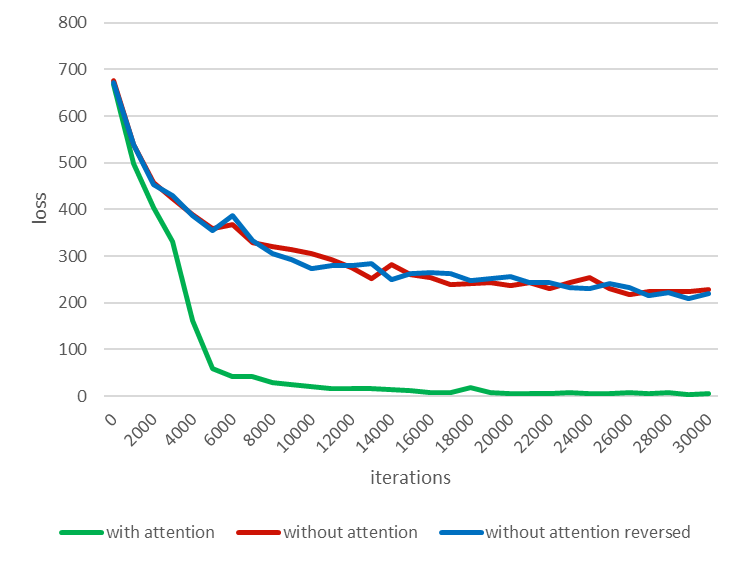
\includegraphics[width=0.9\linewidth]{attention_chart}
\caption{Line chart showing the loss of different models over time.}
\label{attention_chart}
\end{figure}

% Table with eval

Of course it can also be asked if the attention mechanism is necessary for the model, after all it increases complexity and training duration. To test this, the model was constructed without an attention mechanism on top of the decoder. This model was then trained twice, once with the same input the regular model got and once with the input reversed. The reversion of the input is a technique proposed in \cite{seq2seq}, the idea being to introduce more short term dependencies while the average distance of the dependencies stays the same. This is not necessary for the regular model because the attention mechanism allows the model to take a peek of the encoder state at any given timestep.

Figure \ref{attention_chart} shows the loss of the different models as a function over iterations.

\subsection{RNN vs. LSTM (vs. GRU)}

\begin{figure}[p]
\centering
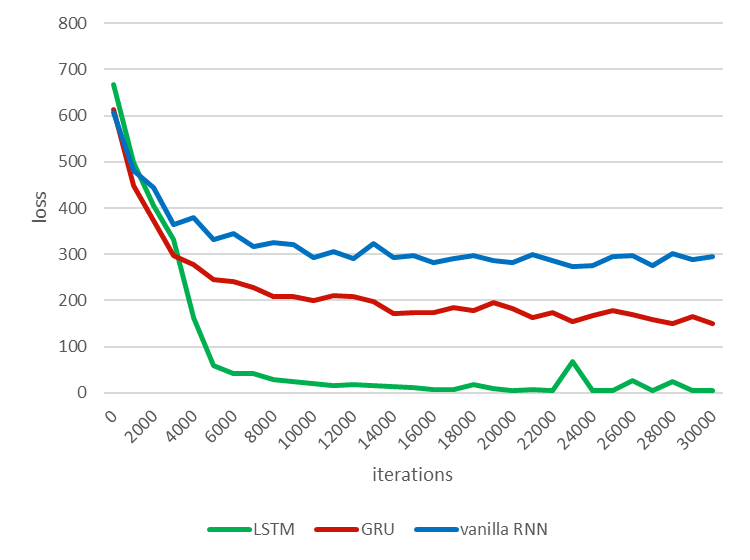
\includegraphics[width=0.9\linewidth]{cell_type_chart}
\caption{Line chart showing the loss of different models over time.}
\label{cell_type_chart}
\end{figure}

\section{Error analysis}

\subsection{Uncorrupted}

similar characters. *(42), +(43)

incorrect switching of lines

tolerance: 79.6\%

wrong switch: 4.1\%

\subsection{Brackets}

balanced brackets: 77.2\%

matching brackets: 76.9\%

\subsection{Semicolon}

tolerance: 81.7\%

wrong switch: 2.9\%

correct number of semicolons: 97.0\%

\subsection{Variable}

\begin{figure}[p]
\centering
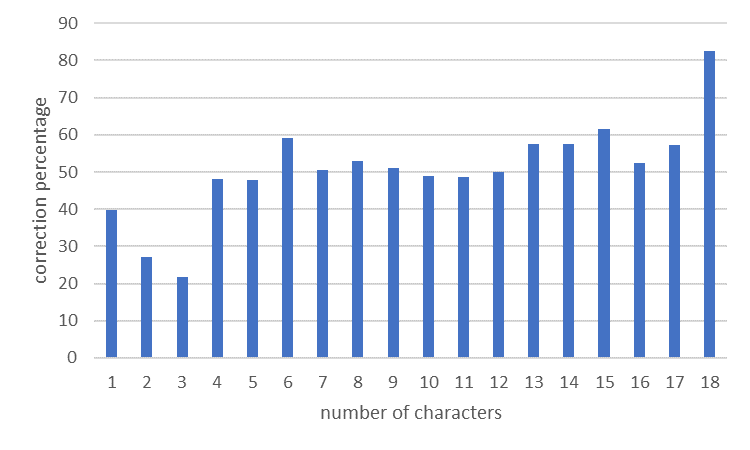
\includegraphics[width=0.9\linewidth]{variables_chart}
\caption{Correction percentage for variables evaluated for different lengths. Only lengths with more than 10 examples were considered.}
\label{variables_chart}
\end{figure}

\subsection{Return type}

different percentages

\subsection{Switch}

\begin{table}[h]
\begin{tabular}{ | m{1cm} | m{1cm} | m{1cm} | m{1cm} | }
  \hline
  \(\leftrightarrow\) & VC & MI & AS \\
  \hline
  \hline
  VC & - & 53.3 & \textbf{59.3} \\
  \hline
  MI & 0.0 & - & 13.0 \\
  \hline
  AS & 0.0 & 9.8 & - \\
  \hline
\end{tabular}
\caption{VC = Variable Declaration, MI = method invocation, AS = assignment.}
\label{switch_table}
\end{table}

\section{Showcase}

\begin{table}[p]
\begin{tabular}{ | m{11cm} | }
  \hline
  Uncorrupted \\
  \hline
  {\begin{lstlisting}[style=table]
  public final void enable() {
    FileConfiguration config = new FileConfiguration(NoLagg.plugin);
    config.load();
    this.enable(config);
    config.save();
  }
  \end{lstlisting}} \\
  {\begin{lstlisting}[style=table]
  public final void enable() {
   FileConfiguration config = new FileConfiguration(NoLagg.plugin);
   config.load();
   this.enable(config);
   config.save();
  }
  \end{lstlisting}} \\
  \hline
  \hline
  {\begin{lstlisting}[style=table]
  private Vec4 parseVec4(String s) {
   Scanner snr = new Scanner(s);
   Vec4 res = new Vec4();
   res.x = Float.parseFloat(snr.next());
   res.y = Float.parseFloat(snr.next());
   res.z = Float.parseFloat(snr.next());
   res.w = Float.parseFloat(snr.next());
   return res;
  }
  \end{lstlisting}} \\
  {\begin{lstlisting}[style=table]
  private Vec4 parseVec4(String s) {
   Scanner snr = new Scanner(s);
   Vec4 res = new Vec4();
   res.x = Float.parseFloat(snr.next());
   res.y = Float.parseFloat(snr.next());
   res.$y$ = Float.parseFloat(snr.next());
   res.w = Float.parseFloat(snr.next());
   return res;
  }
  \end{lstlisting}} \\
  \hline
\end{tabular}
\caption{Example}
\label{uncorrupted_showcase_table}
\end{table}

\begin{table}[p]
\begin{tabular}{ | m{11cm} | }
  \hline
  Brackets \\
  \hline
  {\begin{lstlisting}[style=table]
  int pop(int numBits) $_$
   int i = getLeadingAsInt(numBits);
   truncate(numBits);
   return i;
  }
  \end{lstlisting}} \\
  {\begin{lstlisting}[style=table]
  int pop(int numBits) ^{^
   int i = getLeadingAsInt(numBits);
   truncate(numBits);
   return i;
  }
  \end{lstlisting}} \\
  \hline
  \hline
  {\begin{lstlisting}[style=table]
  protected void outlineShape(Graphics graphics, Rectangle bounds) {
   PointList pl = setupPoints$_$bounds);
   graphics.drawPolygon(pl);
   int add = graphics.getLineWidth() / 2;
   graphics.drawOval(new Rectangle(ovalX, ovalY, ovalD + add, ovalD + add));
  }
  \end{lstlisting}} \\
  {\begin{lstlisting}[style=table]
  protected void outlineShape(Graphics graphics, Rectangle bounds) {
   PointList pl = setupPointsbounds$($);
   graphics.drawPolygon(pl);
   int add = graphics.getLineWidth() / 2;
   graphics.drawOval(new Rectangle(ovalX, ovalY, ovalD + add, ovalD + add));
  }
  \end{lstlisting}} \\
  \hline
\end{tabular}
\caption{Example}
\label{brackets_showcase_table}
\end{table}

\begin{table}[p]
\begin{tabular}{ | m{11cm} | }
  \hline
  Semicolons \\
  \hline
  {\begin{lstlisting}[style=table]
  @Override
  public Method run() {
   try {
    final Method mtd = clazz.getMethod("writeReplace")$_$
    mtd.setAccessible(true);
    return mtd;
   } catch (NoSuchMethodException e) {}
   return null;
  }
  \end{lstlisting}} \\
  {\begin{lstlisting}[style=table]
  @Override
  public Method run() {
   try {
    final Method mtd = clazz.getMethod("writeReplace")^;^
    mtd.setAccessible(true);
    return mtd;
   } catch (NoSuchMethodException e) {}
   return null;
  }
  \end{lstlisting}} \\
  \hline
  \hline
  {\begin{lstlisting}[style=table]
  public void test_hashCode() {
   ExternalIdWithDates d1a = ExternalIdWithDates.of(IDENTIFIER, VALID_FROM, VALID_TO);
   ExternalIdWithDates d1b = ExternalIdWithDates.of(IDENTIFIER, VALID_FROM, VALID_TO);
   assertEquals(d1a.hashCode(), d1b.hashCode())$_$
  }
  \end{lstlisting}} \\
  {\begin{lstlisting}[style=table]
  public void test_hashCode() {
   ExternalIdWithDates d1a = ExternalIdWithDates.of(IDENTIFIER, VALID_TO);
   ExternalIdWithDates d1b = ExternalIdWithDates.of(IDENTIFIER, VALID_TO);
   assertEquals(d1a.hashCode(), d1b.hashCode());
   $assertEquals(d1a.hashCode(), d1b.hashCode());$
  }
  \end{lstlisting}} \\
  \hline
\end{tabular}
\caption{Example}
\label{semicolon_showcase_table}
\end{table}

\begin{table}[p]
\begin{tabular}{ | m{11cm} | }
  \hline
  Variable \\
  \hline
  {\begin{lstlisting}[style=table]
  private boolean validateOrder(InteractionOperand interactionOperand) {
   orderedFragments = $interactionOpernd$.getFragments();
   computeConstraints();
   return reorderFragmentsInAValidTrace();
  }
  \end{lstlisting}} \\
  {\begin{lstlisting}[style=table]
  private boolean validateOrder(InteractionOperand interactionOperand) {
   orderedFragments = ^interactionOperand^.getFragments();
   computeConstraints();
   return reorderFragmentsInAValidTrace();
  }
  \end{lstlisting}} \\
  \hline
  \hline
  {\begin{lstlisting}[style=table]
  @Override
  public void mouseReleased(MouseEvent e) {
   popup.setVisible(false);
   String colorText = "RGB = " + buttonColor.getRed() + ", " + buttonColor.getBreen() + ", " + buttonColor.getBlue();
   this.setText($colrText$);
   this.firePropertyChange(COLOR_CHANGE, previousColor, buttonColor);
  }
  \end{lstlisting}} \\
  {\begin{lstlisting}[style=table]
  @Override
  public void mouseReleased(MouseEvent e) {
   popup.setVisible(false);
   String colorText = "RGB = " + buttonColor.getRed() + ", " + buttonColor.getBreen() + ", " + buttonColor.getBlue();
   this.setText($colrText$);
   this.firePropertyChange(COLOR_CHANGE, previousColor, buttonColor);
  }
  \end{lstlisting}} \\
  \hline
\end{tabular}
\caption{Example}
\label{variable_showcase_table}
\end{table}

\begin{table}[p]
\begin{tabular}{ | m{11cm} | }
  \hline
  Return type \\
  \hline
  {\begin{lstlisting}[style=table]
  @Override
  public $void$ toString() {
   if (eIsProxy()) return super.toString();
   StringBuffer result = new StringBuffer(super.toString());
   result.append(" (name: ");
   result.append(name);
   result.append(')');
   return result.toString();
  }
  \end{lstlisting}} \\
  {\begin{lstlisting}[style=table]
  @Override
  public ^String^ toString() {
   if (eIsProxy()) return super.toString();
   StringBuffer result = new StringBuffer(super.toString());
   result.append(" (name: ");
   result.append(name);
   result.append(')');
   return result.toString();
  }
  \end{lstlisting}} \\
  \hline
  \hline
  {\begin{lstlisting}[style=table]
  @Override
  public $void$ evaluate(final Double...ts) {
   Validate.isTrue(ts.length == 2);
   final double tau = ts[0];
   final double s = ts[1];
   final double t = maturity - tau;
   final double temp = vol * Math.pow(s, beta) * localVol.getVolatility(t, s);
   return -0.5 * temp * temp;
  }
  \end{lstlisting}} \\
  {\begin{lstlisting}[style=table]
  @Override
  public $Validate$ evaluate(final Double...ts) {
   $>$final double tau = ts[0];
   $>$Validate.isTrue(ts.length == 2);
   final double s = ts[1];
   final double t = maturity - tau;
   final double temp = vol * Math.pow(s, beta) * localVol.getVolatility(t, s);
   return -0.5 * temp * temp;
  }
  \end{lstlisting}} \\
  \hline
\end{tabular}
\caption{Example}
\label{return_type_showcase_table}
\end{table}

\begin{table}[p]
\begin{tabular}{ | m{11cm} | }
  \hline
  Switch \\
  \hline
  {\begin{lstlisting}[style=table]
  protected void disposeElementInfo(Object element, ElementInfo info) {
   if (info instanceof ResourceSetInfo) {
    $>$resourceSetInfo.dispose();
    $>$ResourceSetInfo resourceSetInfo = (ResourceSetInfo) info;
   }
   super.disposeElementInfo(element, info);
  }
  \end{lstlisting}} \\
  {\begin{lstlisting}[style=table]
  protected void disposeElementInfo(Object element, ElementInfo info) {
   if (info instanceof ResourceSetInfo) {
    ^>^ResourceSetInfo resourceSetInfo = (ResourceSetInfo) info;
    ^>^resourceSetInfo.dispose();
   }
   super.disposeElementInfo(element, info);
  }
  \end{lstlisting}} \\
  \hline
  \hline
  {\begin{lstlisting}[style=table]
  private void resolveEntry(Entry < K, T > entry) {
   $>$entry.isResolved = true;
   $>$resolved.add(entry);
   resolved(entry);
  }
  \end{lstlisting}} \\
  {\begin{lstlisting}[style=table]
  private void resolveEntry(Entry < K, T > entry) {
   $>$entry.isResolved = true;
   $>$resolved.add(entry);
   resolved(entry);
  }
  \end{lstlisting}} \\
  \hline
\end{tabular}
\caption{Example}
\label{switch_showcase_table}
\end{table}
